\documentclass[11pt]{article}

% Do not use packages other than asp2014. 
\usepackage{asp2014}

% TO BE REMOVED !
\usepackage{color}

\aspSuppressVolSlug
\resetcounters

\markboth{P.~Bacon, V.~Savchenko, E.~Chassande-Mottin and P.~Laurent}{P.~Bacon, V.~Savchenko, E.~Chassande-Mottin and P.~Laurent}

\begin{document}

\title{Prospects about X- and gamma-ray counterparts of gravitational wave signals with INTEGRAL.}
\author{P.~Bacon, V.~Savchenko, E.~Chassande-Mottin and P.~Laurent}
\affil{APC, AstroParticule et Cosmologie, Universite Paris Diderot, CNRS/IN2P3, CEA/Irfu,
Observatoire de Paris, Sorbonne Paris Cite, Paris, France; \email{philippe.bacon@apc.in2p3.fr}}

%% This section is for ADS Processing.  There must be one line per author.
\paperauthor{P.~Bacon}{philippe.bacon@apc.in2p3.fr}{}{Laboratoire Astroparticule et Cosmologie}{Physics}{Paris}{Ile-de-France}{75013}{France}
\paperauthor{V.~Savchenko}{savchenk@apc.in2p3.fr}{}{Laboratoire Astroparticule et Cosmologie}{Physics}{Paris}{Ile-de-France}{75013}{France}
\paperauthor{E.~Chassande-Mottin}{ecmn@apc.in2p3.fr}{}{Laboratoire Astroparticule et Cosmologie}{Physics}{Paris}{Ile-de-France}{75013}{France}
\paperauthor{P.~Laurent}{philippe.laurent@apc.in2p3.fr}{}{Laboratoire Astroparticule et Cosmologie}{Physics}{Paris}{Ile-de-France}{75013}{France}

\begin{abstract}
%	By extrapolating the number of detections made during the first
%   	LIGO science run, tenths of gravitational wave signals from binary
%   	black hole mergers are anticipated in upcoming LIGO Virgo science
%   	runs. Finding an electromagnetic counterpart to compact binary
%   	merger events would be a landmark discovery. The search for such
%   	counterpart is challenging for a number of reasons, such as the
%   	poor resolution of source position reconstruction from the
%   	gravitational wave observations alone, and the weakness of the
%   	expected electromagnetic signal. In this poster, we evaluate the
%   	ability of current wide-field X- and gamma-ray telescopes aboard
%   	INTEGRAL to find such counterparts. We present the result of an
%   	end-to-end simulation for estimating the fraction of the sources
%   	that can be followed up, and the fraction of counterparts that can
%   	be detected based on different models.
    By extrapolating the number of detections made during the first
    LIGO science run, tenths of gravitational wave signals from binary
    	black hole mergers are anticipated in upcoming LIGO Virgo science
    	runs. Finding an electromagnetic counterpart from compact binary
    	merger events would be a capital achievement if we want to solve 
    	some raised issues from the September 2015 event. We evaluate the
   	ability of current wide-field X- and gamma-ray telescopes aboard
   	INTEGRAL to find such counterparts thanks to an end-to-end simulation
   	for estimating the fraction of the sources that can be followed up and/or
   	detected. \\
\end{abstract}

\textcolor{blue}{Have to be changed in the future version of the proceeding} \\
\textcolor{magenta}{Can be removed or reformulated in the future version of the proceeding} \\
 
%\section*{Motivations}

%On Sep 14 2015, the two LIGO interferometers made the first direct detection of
%gravitational waves (GW). A next step would be to detect an electromagnetic (EM)
%counterpart associated to a GW event. This would inaugurate a new,
%multimessenger era in the astronomy history. We address the question of the
%joint detectability of GW events by Advanced LIGO, and
%associated EM events at high-energies by the INTEGRAL mission. We produce an
%end-to-end simulation of the search for gravitational-waves from binary
%neutron star mergers and follow-up observation seeking a possible
%electromagnetic counterpart at high-energies. This study is similar to the
%one done in \citep{2016arXiv160606124P} with Fermi.

On September 14, 2015, the two LIGO interferometers realized the first direct detection of
gravitational waves (GW). A next achievement would be to attach an electromagnetic (EM)
counterpart to a GW event. We thus address the question of the joint detectability 
of GW events by Advanced LIGO, and associated EM events at high-energies by the 
INTEGRAL mission. This study is similar to the one done in \citep{2016arXiv160606124P} with Fermi.

\section*{Monte-Carlo simulation of gravitational-wave events from neutron-star binary mergers}

We start with a simulated catalogue of 6 millions Milky Way-like galaxies
distributed to $z\sim 0.12$. To those galaxies, we associate binary neutron star
(BNS) mergers with mass distribution and rate of R=$23.5 M\mathrm{yr}^-3$ per galaxy
according to Model A (solar metallicity) of
\citep{2012ApJ...759...52D}. This results in a population of 14\,000
mergers for a $100$ year simulation.

\begin{center}[!ht]
   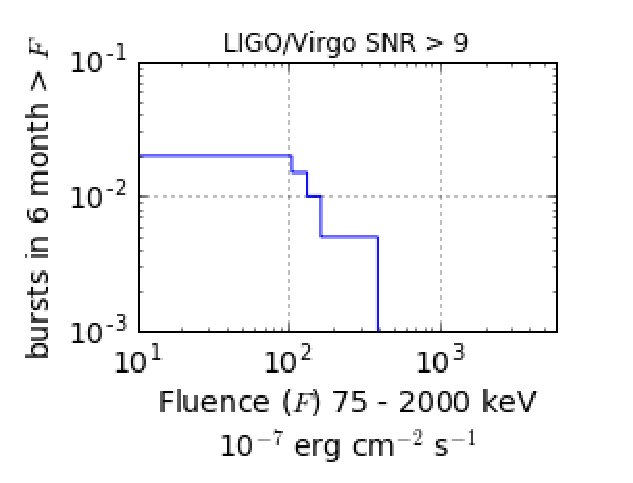
\includegraphics[scale=.7]{P7-1_f1.eps}
   \textcolor{blue}{Fig.1 : remove mass distribution.}
\end{center}

We simulate GW signals corresponding to the binary mergers (using model
``TaylorT4'') and inject them into Gaussian noise coloured according to the
``optimistic'' power-spectral density anticipated for the 2nd LIGO/Virgo run O2
\citep{2016LRR....19....1A}. \textcolor{blue}{We select signals with $\mathrm{SNR}_{\mathrm{combined}} > 9$.}
corresponding to a false-alarm rate $\mathrm{FAR} < 1/\mathrm{month}$. \textcolor{blue}{The
average range BNS is 126 Mpc for this selection.}

This results in \textcolor{blue}{232 selected merger signals over 100 years which corresponds to
$\sim 1$ merger over the 6-month duration of O2.} We distribute those events
randomly in time over the expected period of O2 from Nov 2016 to May 2017. We
recover GW signals using matched-filtering techniques and reconstruct the
posterior skymaps giving the position of the source using the BAYESTAR pipeline
\citep{2016PhRvD..93b4013S}.  \textcolor{blue}{With two detectors only, the position uncertainty is
large and contained in a window of 700--2000 square degrees.}

\section*{Electromagnetic emission model from neutron-star binary mergers}

Compact binary mergers involving at least one neutron star are considered to be
plausible progenitors of short gamma-ray bursts (GRB). Short GRBs is a
subset of the whole GRB population with duration shorter than $\sim$2
seconds. Short GRBs have also a harder spectrum. Prompt emission is attributed
to dissipation within the collimated ultra-relativistic jet and is therefore
strongly beamed. It is followed by slowly decaying afterglow, observed from
radio to GeV, produced by the interaction between the ejecta and the ambient
medium surrounding the GRB progenitor. Afterglow emission is originally also
strongly beamed, but as the outflow decelerates, the emission becomes
progressively more isotropic.

In our simulation we assume that every BNS merger is associated with a short
gamma-ray burst. We simulate synthetic prompt GRB and a hard X-ray afterglow,
assuming the following simplified model. \\

%\subsection*{Prompt emission}

We model the prompt emission spectrum by the cut-off power-law model. This
model is a variant of the Band model \citep{1993ApJ...413..281B} \textcolor{magenta}{where high-energies have
been suppressed because they are generally not well constrained by the
observations.} For simplicity we assume the same prompt emission spectrum
for all synthetic GRB, with $\alpha_{\mathrm{BAND}} = - 0.5$ and
$E_{\mathrm{peak}} = 600$ \, keV, close to the average short GRB spectrum
observed by Fermi/GBM \citep{2014ApJS..211...12G}.   
%\ECM{Not clear: In the case of short
%  GRBs, the slope above the peak energy is not well constrained, and the
%  spectrum can be well described by a cutoff power-law. -- Would this be
%  correct?: Above the peak energy, the spectrum can be well described by a
%  cut-off power-law, although the slope is not well constrained.} 
We also assume
fixed duration of the prompt emission of $1 \, s$ and fixed isotropic equivalent
luminosity of $10^{50}~$erg~cm$^{-2}$~s$^{-1}$.

The principal source of uncertainty on rate of GRB detections associated with
the BNS mergers is the beaming factor of the prompt emission. We assume a fixed
beaming angle of 10 degrees \textcolor{blue}{when $\Gamma_{0} = 200$ according to what we have said?}. This angle is roughly compatible with the
observations of the total short GRB rate inferred from our BNS population. \\

%\subsection*{Hard X-ray afterglows}

We assume that every BNS merger produces a hard X-ray afterglow. Although
afterglows in the hard X-rays are rarely observed, it is not unreasonable to
assume that they are as frequent as gamma-rays, but observed much less
frequently due to observational limitations.

There are indications that such afterglows are present in the most luminous GRBs
occurring about once in few months (2\% of the sky observed by INTEGRAL).  When
hard X-ray afterglows are observed, INTEGRAL observations reveals very high
SNR. \textcolor{magenta}{For instance, GRB120711A was seen in INTEGRAL/ISGRI and JEM-X for about 8
hours \citep{2014A&A...567A..84M}. The bright hard X-ray emission afterglow found to
be related to the bright gamma-ray afterglow, observed by Fermi/LAT in the
energy range above 100 MeV. In particular, it had the same spectrum, power-law
with a slope of -2.}

\textcolor{magenta}{We assume a spectrum similar to GRB120711A, but rescaled to the total EM
luminosity of a typical short GRB - $10^{50}~$erg$^{-2}~$s$^{-1}$.} We extrapolate
this spectrum to the off-axis case using Model~I in \citep{2016arXiv160606124P}.

\section*{The INTEGRAL mission and possible follow-up strategies}

% LINK : http://www.cosmos.esa.int/web/integral/instruments-ibis
%        http://www.cosmos.esa.int/web/integral/instruments-spi

The INTEGRAL satellite carries a combination of pointing instruments, covering
wide energy range from 3 keV to 10 MeV (ISGRI, PICsIT, JEM-X, and SPI) with
field of view up to 900 deg$^2$. Active follow-up: We assume that every
GW alerts reported by LIGO/Virgo is followed by INTEGRAL pointings. Typical
latency of INTEGRAL observation is about 1 day but may be lower in some
circumstances. We compute the flux at several moments of time, and compare it
with ISGRI sensitivity in 100~ks observation. Passive follow-up: In
addition, INTEGRAL/SPI-ACS and IBIS are capable of detecting bright transients
from every sky direction.

\section*{Results}

%\subsection*{Prompt -- Passive follow-up}

\begin{figure}
	\centering
    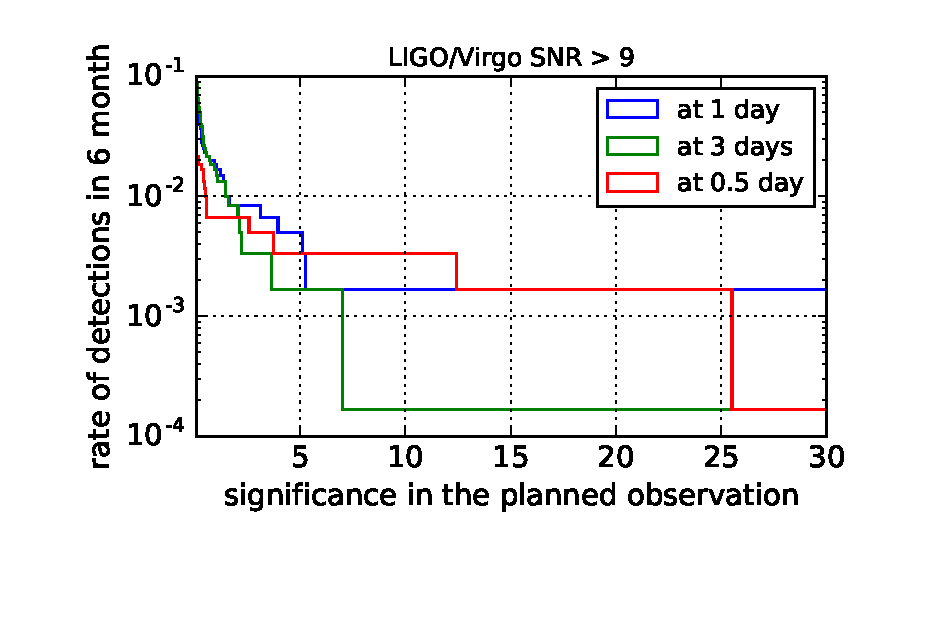
\includegraphics[scale=.6]{P7-1_f4.eps}
    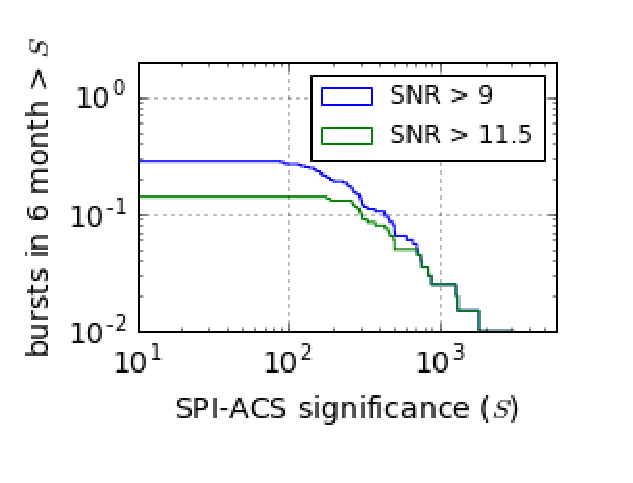
\includegraphics[scale=.6]{P7-1_f5.eps}
    \caption{(\textit{Left}) Cumulative distribution of the
      detected fluences by INTEGRAL in the LIGO/Virgo O2
      run.(\textit{Right}) Cumulative distribution of the significance
      in the INTEGRAL/SPI-ACS instrument. \textcolor{blue}{Change figures}}
    \label{fluence_significance}
\end{figure}

Choosing an isotropic sky distribution for the passive follow-up emission (passive follow-up) 
of our GW events, \textcolor{blue}{we show that
in every case where the Earth is within the GRB emission cone,
INTEGRAL detects prompt emission with significance at least 50~sigma.
The rate of detection is 0.5 in the 6 months of O2 for GW alerts ($\mathrm{SNR} \geq 9$) 
and 0.1 in 6 months  in the case of 4-sigma GW events (SNR = 11.5).} \\

%\subsection*{Afterglow -- Instrument repointing}

If we want to follow-up the afterglow emission, we will need to re-point the on-board instruments.
INTEGRAL can point only to a fraction of the GW localization region. For each
event we compute the total localization probability within the observable
region, and find that \textcolor{blue}{in 40\% of the cases 80\% of the localization is
observed. However, if the complete available region is followed up every
time, in total 80\% of the true source locations are covered.}

\begin{figure}[!ht]
	\centering
  	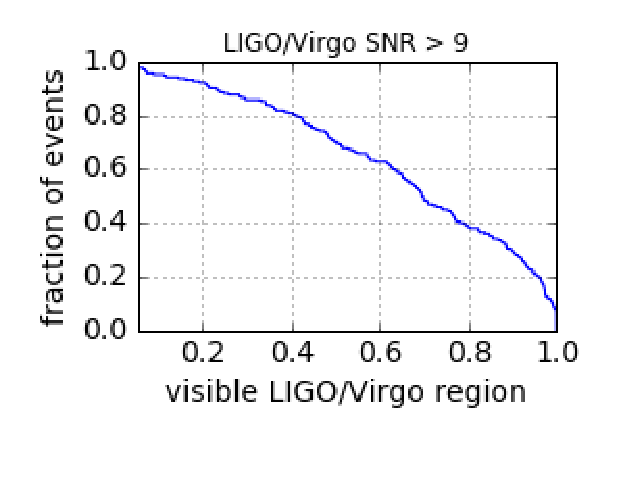
\includegraphics[scale=.5]{P7-1_f6.eps}
  	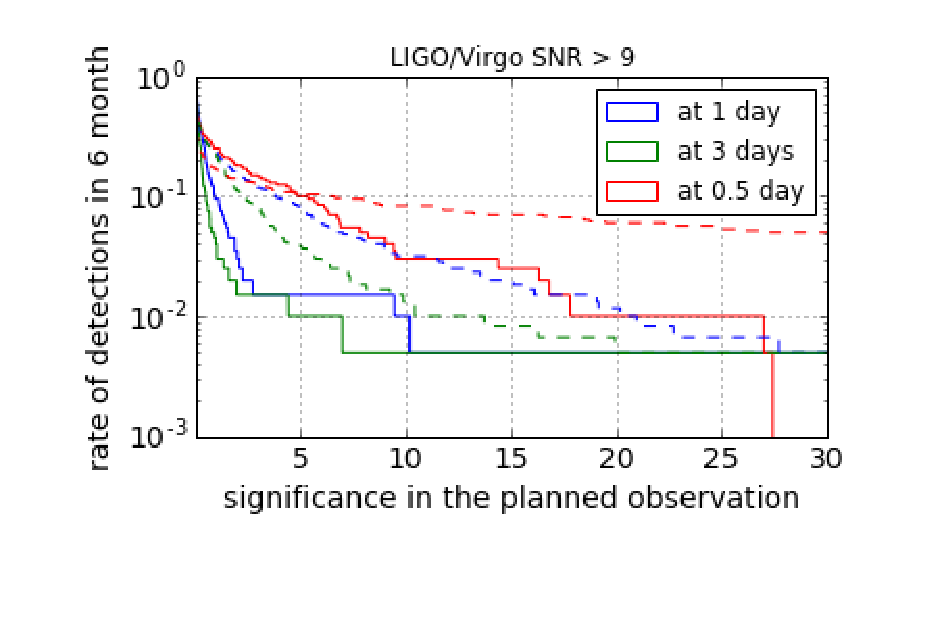
\includegraphics[scale=.4]{P7-1_f7.eps}

  	\caption{(\textit{Left}) Cumulative distribution of the
    fraction of the LIGO/Virgo localization region accessible to
    INTEGRAL pointed follow-up observation in the LIGO/Virgo O2
    run. (\textit{Right}) Significance distribution on detected
    sources depending on time delay after the prompt emission. Dotted
    lines correspond to the model assuming realistic distribution of short GRB luminosities. \textcolor{blue}{Change figures}}
    \label{covered_region}
\end{figure}

\textcolor{blue}{We find that the expected rate of 5~sigma detections is only about
0.01 events in 6 months of O2. We explore also another
possibility, that 10\% of the events launch much more energetic
outflow, in agreement with luminosities observed in real short
GRBs. In this case we expect about 0.1 events seen in 6 months.}

We stress that the afterglow prediction is particularly sensitive to
assumptions on rather uncertain source model, and we assume only
one, yet realistic, option.

\vspace{10mm}
\noindent {\normalsize \textbf{Acknowledgements}}

%----------------------------------------------------------------------------------------
%	ACKNOWLEDGEMENTS
%----------------------------------------------------------------------------------------

{\linespread{0.1} \footnotesize This research was supported European Union´s Horizon 2020 research and
  innovation programme under grant agreement No 653477. The authors would like
  to thank the LIGO Scientific Collaboration and Virgo Collaboration for giving
  access to the simulation software used here, Barbara Patricelli for sharing
  her simulations with us.}

%----------------------------------------------------------------------------------------
%	REFERENCES
%----------------------------------------------------------------------------------------

{\footnotesize
\bibliographystyle{asp2014.bst} % Plain referencing style
\bibliography{P7-1.bib} % Use the example bibliography file sample.bib
}

\end{document}